\section{Modeling}

\begin{definition}[\textit{System}]
    A system denoted by $S$ refers to a physical entity designed to convert inputs (causes) into outputs (effects).
\end{definition}
\begin{definition}[\textit{Model}]
    A model, symbolized as $M$, constitutes a mathematical description of a system.
\end{definition}

\begin{figure}[H]
    \centering
    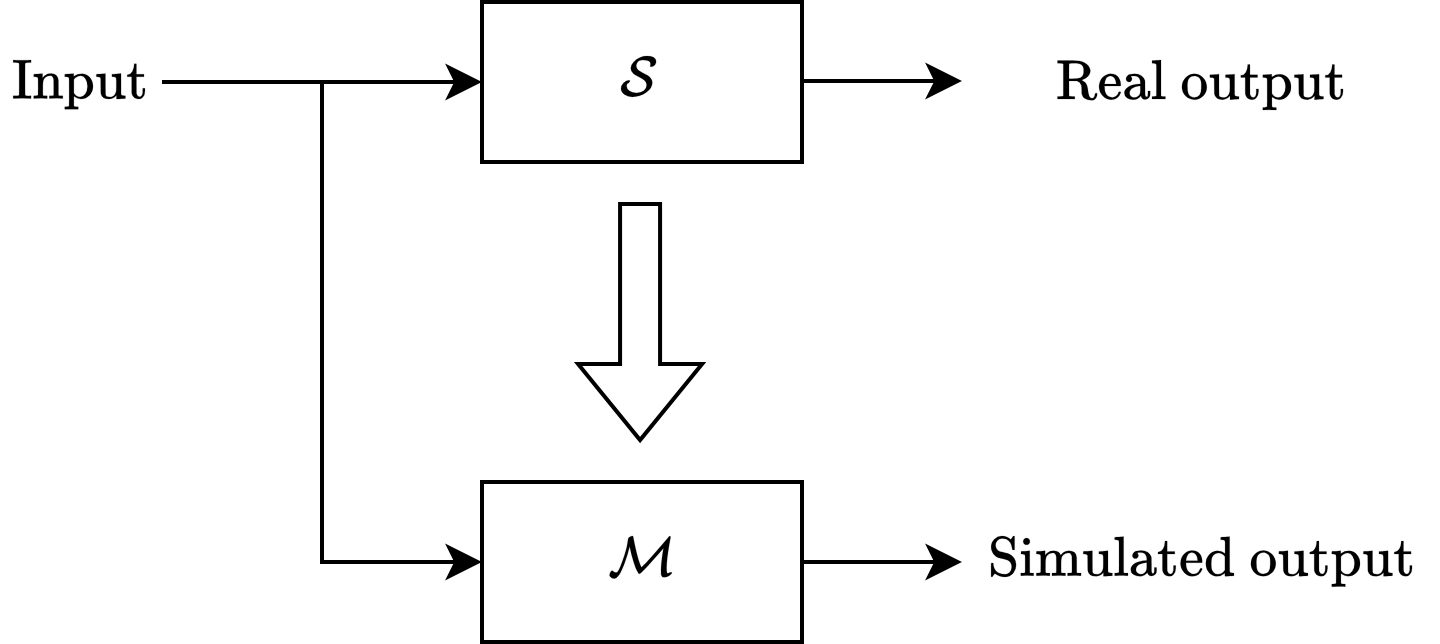
\includegraphics[width=0.5\linewidth]{images/model.png}
    \caption{Visual representation of system and model}
\end{figure}

A model can be constructed through various methodologies:
\begin{enumerate}
    \item \textit{White-box modeling}: this approach relies on established physical laws or existing knowledge. 
        The resultant model is typically generalizable, with clear physical interpretations for each variable.
        However, precise knowledge of all parameters beforehand is necessary, making it a costly and time-intensive process. 
        Consequently, it's often impractical for complex systems.
    \item \textit{Black-box} modeling: this method is based on experimental data. 
        Parameters of the model are estimated using statistical relationships derived from the data. 
        It's feasible even without in-depth knowledge of the underlying processes, and it's comparatively faster and less expensive. 
        However, models generated through this method lack physical interpretability and may not be universally applicable; changes in the system often necessitate repeating the experiment.
\end{enumerate}

\begin{example}
    Consider a block with mass $m$ and a spring with an elastic constant $k$. 
    \begin{figure}[H]
        \centering
        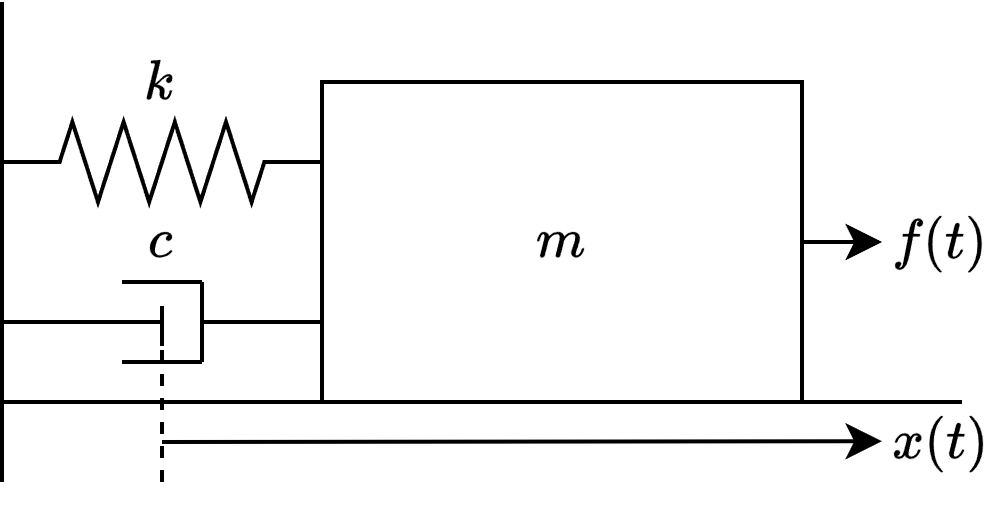
\includegraphics[width=0.45\linewidth]{images/system.png}
    \end{figure}
    In white-box modeling, precise values of parameters such as $m$, $k$, and $c$ are required.
    With this information, the following model can be utilized:
    \[m\ddot x(t)=f(t)-c\dot x(t)-kx(t)\]
    
    On the other hand, black-box modeling necessitates understanding the relationship between inputs and outputs to derive the model. 
    In this scenario, the model obtained is: 
    \[x(t)=-a_1x(t-1)-a_2x(t-2)+b_0f(t)+b_1f(t-1)+b_2f(t-2)\]
    Here, the parameters are determined from the output-input relationships.
\end{example}

\subsection{Error}
The modeling error, also known as the residual, is calculated as the disparity between the system output and the model output generated with the same input.
\begin{figure}[H]
    \centering
    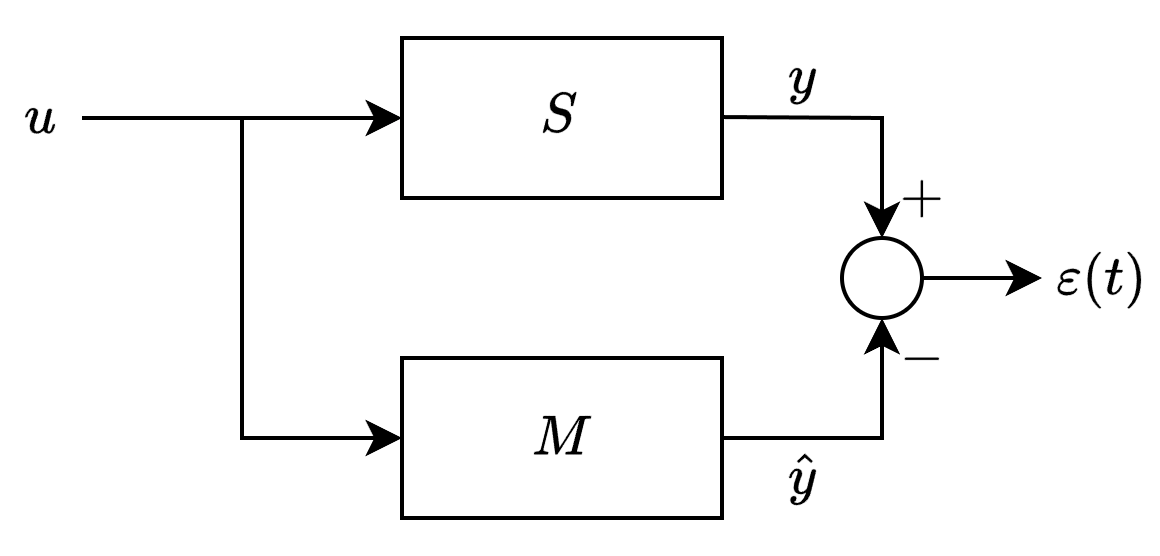
\includegraphics[width=0.5\linewidth]{images/error.png}
\end{figure}
When the outputs exhibit similarity based on certain metrics, it signifies that the model accurately mirrors the dynamics of the system. 
However, if patterns persist within the error graph, it indicates that not all information has been effectively extracted from the data. 
Conversely, if the error graph lacks of patterns, it is termed as white noise, suggesting an inability to extract further meaningful information from the data.
Consequently, a model is deemed complete only when the error demonstrates a completely unpredictable pattern.

\subsection{Classification}
\paragraph*{Static and dynamic}
A system can be categorized as follows:
\begin{itemize}
    \item \textit{Static system}: in this type of system, knowledge of the input variables alone is adequate to determine the output value.
        Classical machine learning primarily addresses the black-box modeling of static systems.
    \item \textit{Dynamic system}: this refers to a system with memory, wherein the past behavior of the output impacts its current value.
\end{itemize}

\begin{example}
    An illustration of a static system is represented by a circuit containing a resistor.
    \begin{figure}[H]
        \centering
        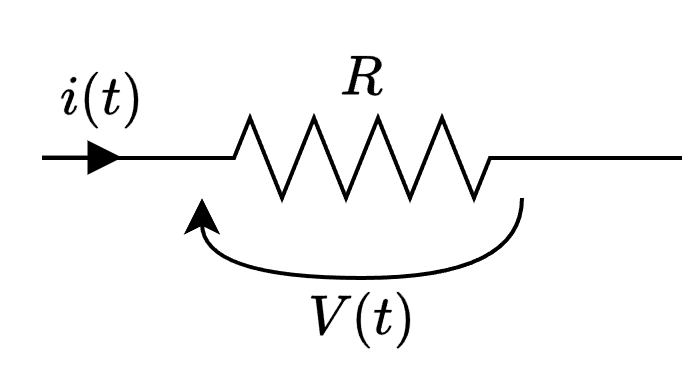
\includegraphics[width=0.35\linewidth]{images/resistor.png}
    \end{figure}
    This system solely relies on the voltage across the resistor at each moment, adhering to Ohm's law:
    \[i(t)=\dfrac{V(t)}{R}\]
    On the other hand, an example of a dynamic system is exemplified by an electrical motor, wherein under certain conditions, even if the input remains constant, the output persists in its evolution.
    \begin{figure}[H]
        \centering
        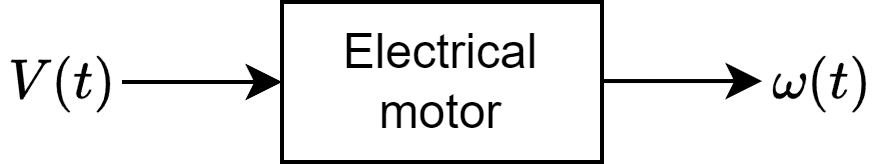
\includegraphics[width=0.5\linewidth]{images/motor.png}
    \end{figure}
\end{example}

\paragraph*{Discrete and continuous}
Systems can be further categorized based on their time description, which can be either discrete or continuous.
Natural and physical phenomena are inherently continuous and are often mathematically described using ordinary differential equations.
On the other hand, discrete systems are mathematically described using difference equations.

However, a computer can only handle a limited amount of data. 
However, computers have limitations in handling data, which necessitates the sampling of signals at discrete intervals with a sampling time $T_s$. 
This ensures that only a finite amount of data is stored at discrete time points $t \cdot T_s$, where $t=1,\dots,N$: 
\[y(t)=y(t \cdot T_s)\]